\documentclass[aspectratio=43]{beamer}

\usepackage[font={scriptsize}]{caption}
\usepackage{graphicx}
\usepackage[utf8]{inputenc}
\usepackage{hyperref}

\title{OpenStack HA - reliability and scalability}
\author{Michał Dulko}
\institute{Intel Technology Poland}
\date{September 26th, 2016}

\begin{document}


\AtBeginSection[]{
  \begin{frame}
  \vfill
  \centering
  \begin{beamercolorbox}[sep=8pt,center,shadow=true,rounded=true]{title}
    \usebeamerfont{title}\insertsectionhead\par%
  \end{beamercolorbox}
  \vfill
  \end{frame}
}

\begin{frame}
\titlepage
\end{frame}

\section{Introduction}

\begin{frame}
    \frametitle{High availability}
    High availability is a characteristic of a system, which aims to ensure an agreed level of operational performance for a higher than normal period.

    There are three principles of system design in high availability engineering:
    \begin{enumerate}
        \item Elimination of single points of failure.
        \item Reliable crossover.
        \item Detection of failures as they occur.
    \end{enumerate}
\end{frame}

\begin{frame}
    \frametitle{OpenStack Architecture}
    \begin{center}
        \begin{figure}
            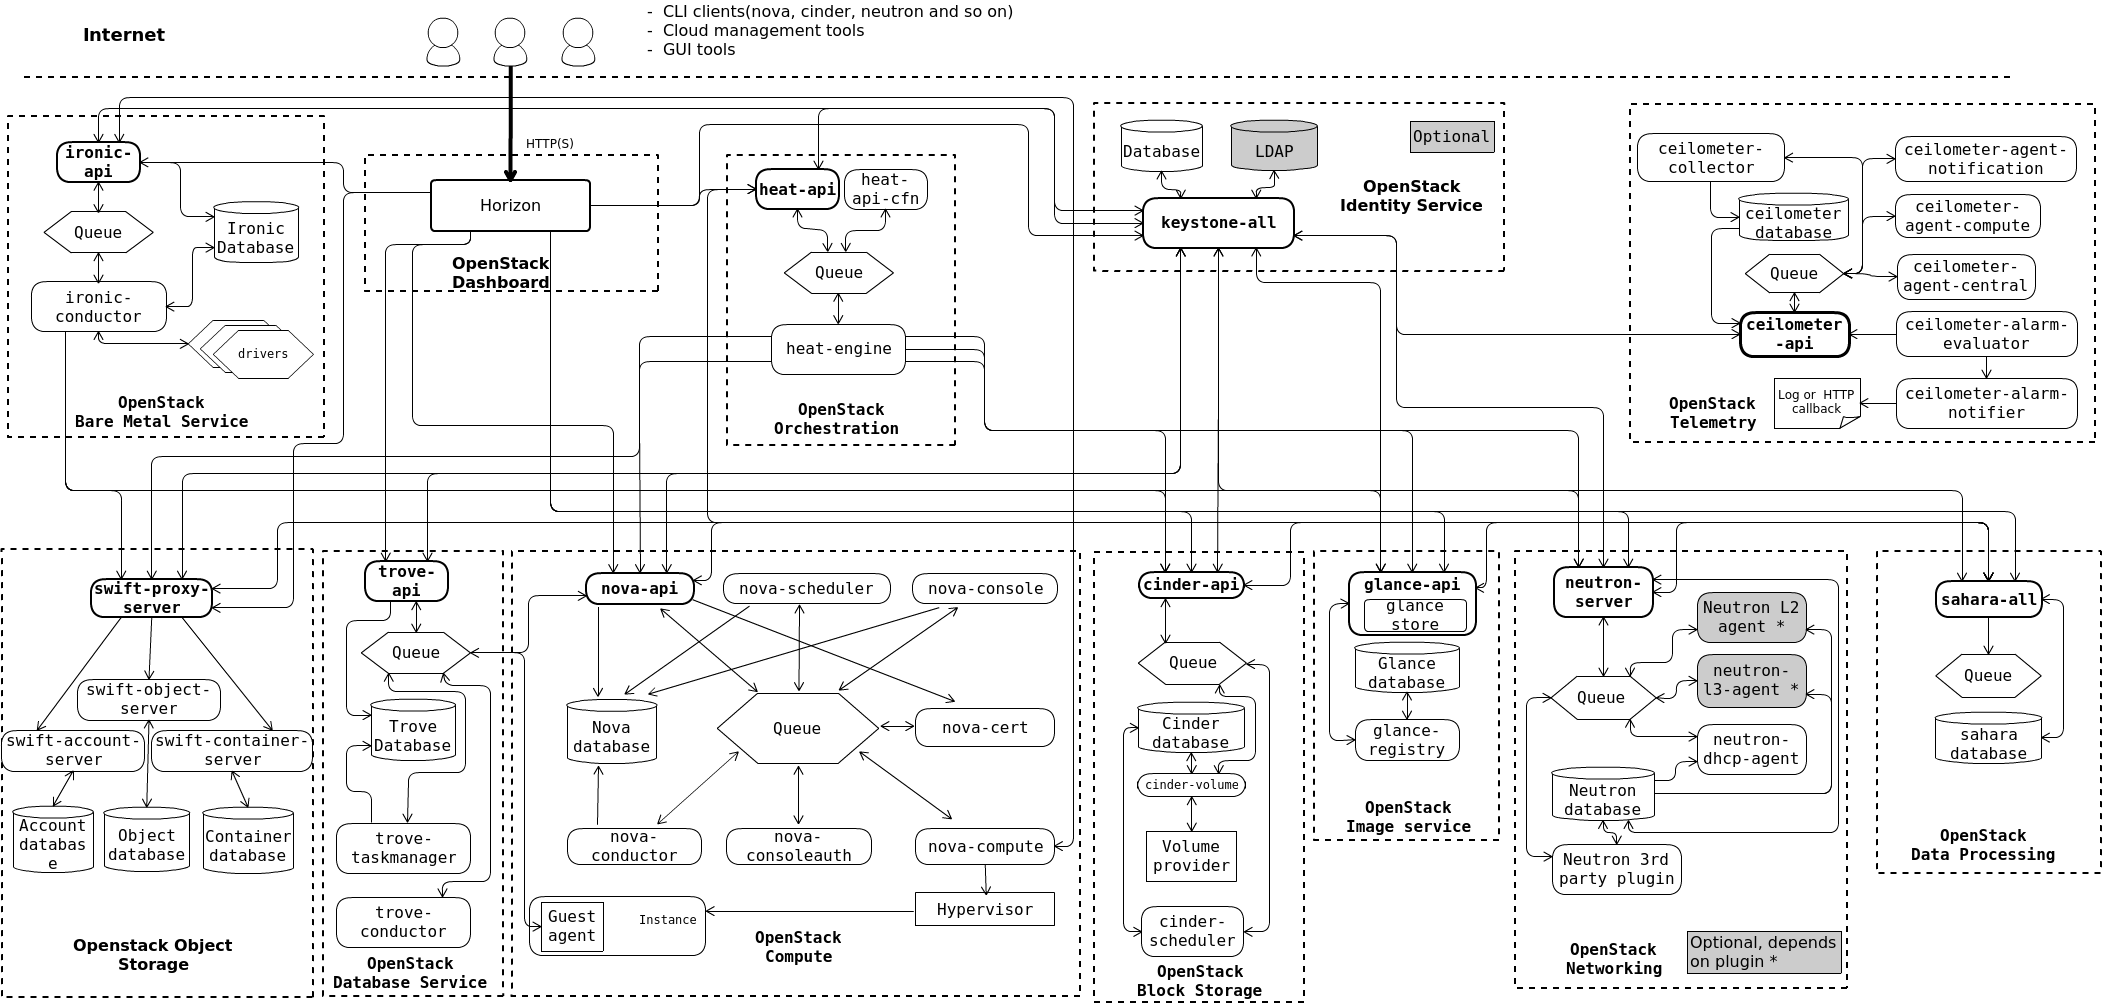
\includegraphics[height=5cm]{images/openstack-arch-kilo-logical-v1.png}

            \tiny{© OpenStack Foundation, Source: http://docs.openstack.org/admin-guide/common/get-started-logical-architecture.html,  Creative Commons Attribution 3.0 License}
        \end{figure}
    \end{center}
\end{frame}

\begin{frame}
    \frametitle{What's actually in there?}
    \begin{center}
        \begin{itemize}
            \pause
            \item OpenStack services (Keystone, Nova, Neutron, Glance, \emph{Cinder}, \emph{Swift}, …)
            \pause
            \item Database (MySQL, PostgreSQL)
            \pause
            \item Message Queue (RabbitMQ, zmq, Apache Kafka))
            \pause
            \item Object storage (Swift, Ceph)
            \pause
            \item Block storage (Ceph, …)
            \pause
            \item \emph{Virtualized networking layer}
        \end{itemize}
    \end{center}
\end{frame}

\section{Shared services}

\begin{frame}
    \frametitle{Database}
    \begin{center}
        \begin{itemize}
            \item Typically - Galera cluster (it's magic!).
            \item Running on 3, 5, 7, … nodes for quorum.
            \item OpenStack is battle-tested on Galera.
        \end{itemize}
    \end{center}
\end{frame}

\begin{frame}
    \frametitle{Message Queue}
    \begin{center}
        \begin{itemize}
            \item Clustered RabbitMQ.
            \item Again running on 3, 5, 7, … nodes for quorum.
            \item Erlang's internal database (Mnesia) is responsible for keeping state consistent.
            \item Running RabbitMQ, especially in HA, is considered non-trivial.
        \end{itemize}
    \end{center}
\end{frame}

\begin{frame}
    \frametitle{Object store}
    \begin{center}
        \begin{itemize}
            \item Ceph
            \begin{itemize}
                \item Has it's own ways of being reliable.
            \end{itemize}
            \pause
            \item Swift
            \begin{itemize}
                \item Runs a "ring", which is basically a consistent hash ring.
                \item You need to make sure to configure Swift to replicate objects.
            \end{itemize}
        \end{itemize}
    \end{center}
\end{frame}

\section{OpenStack services}

\begin{frame}
    \frametitle{Nova architecture}
    \begin{figure}
        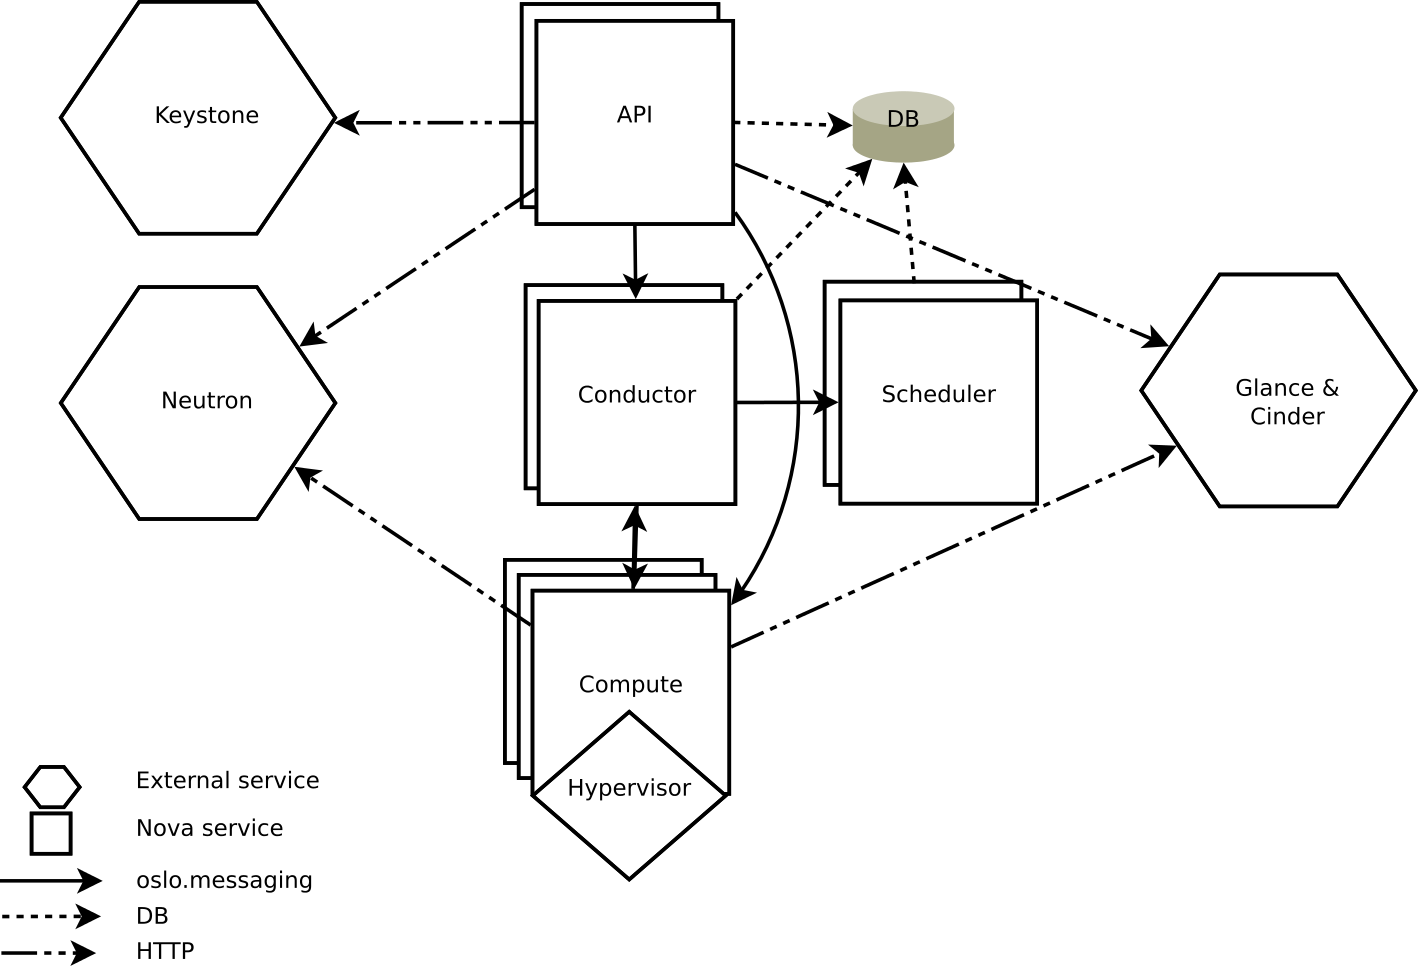
\includegraphics[height=6cm]{images/nova-architecture.png}

        \tiny{© Copyright 2010-present, OpenStack Foundation, Source: http://docs.openstack.org/developer/nova/architecture.html, Apache License 2.0}
    \end{figure}
\end{frame}

\begin{frame}
    \frametitle{OpenStack services types}
    \begin{itemize}
        \item Communication
        \begin{itemize}
            \item REST API services (nova-api, cinder-api, glance-api, Keystone)
            \item Message-queue bound services (\textbf{nova-conductor}, nova-compute, \textbf{cinder-volume})
        \end{itemize}
        \pause
        \item Statefullness
        \begin{itemize}
            \item Stateless, \emph{shared state} (nova-api, \textbf{nova-conductor})
            \item Stateful (\textbf{cinder-volume}, nova-compute)
        \end{itemize}
    \end{itemize}
\end{frame}

\begin{frame}
    \frametitle{REST API services}
    \begin{itemize}
        \item Keystone is run on Apache, rest are either standalone Python services or both.
        \item You're supposed to run them behind HAProxy.
    \end{itemize}
\end{frame}

\begin{frame}
    \frametitle{HAProxy + REST API}
    \begin{center}
        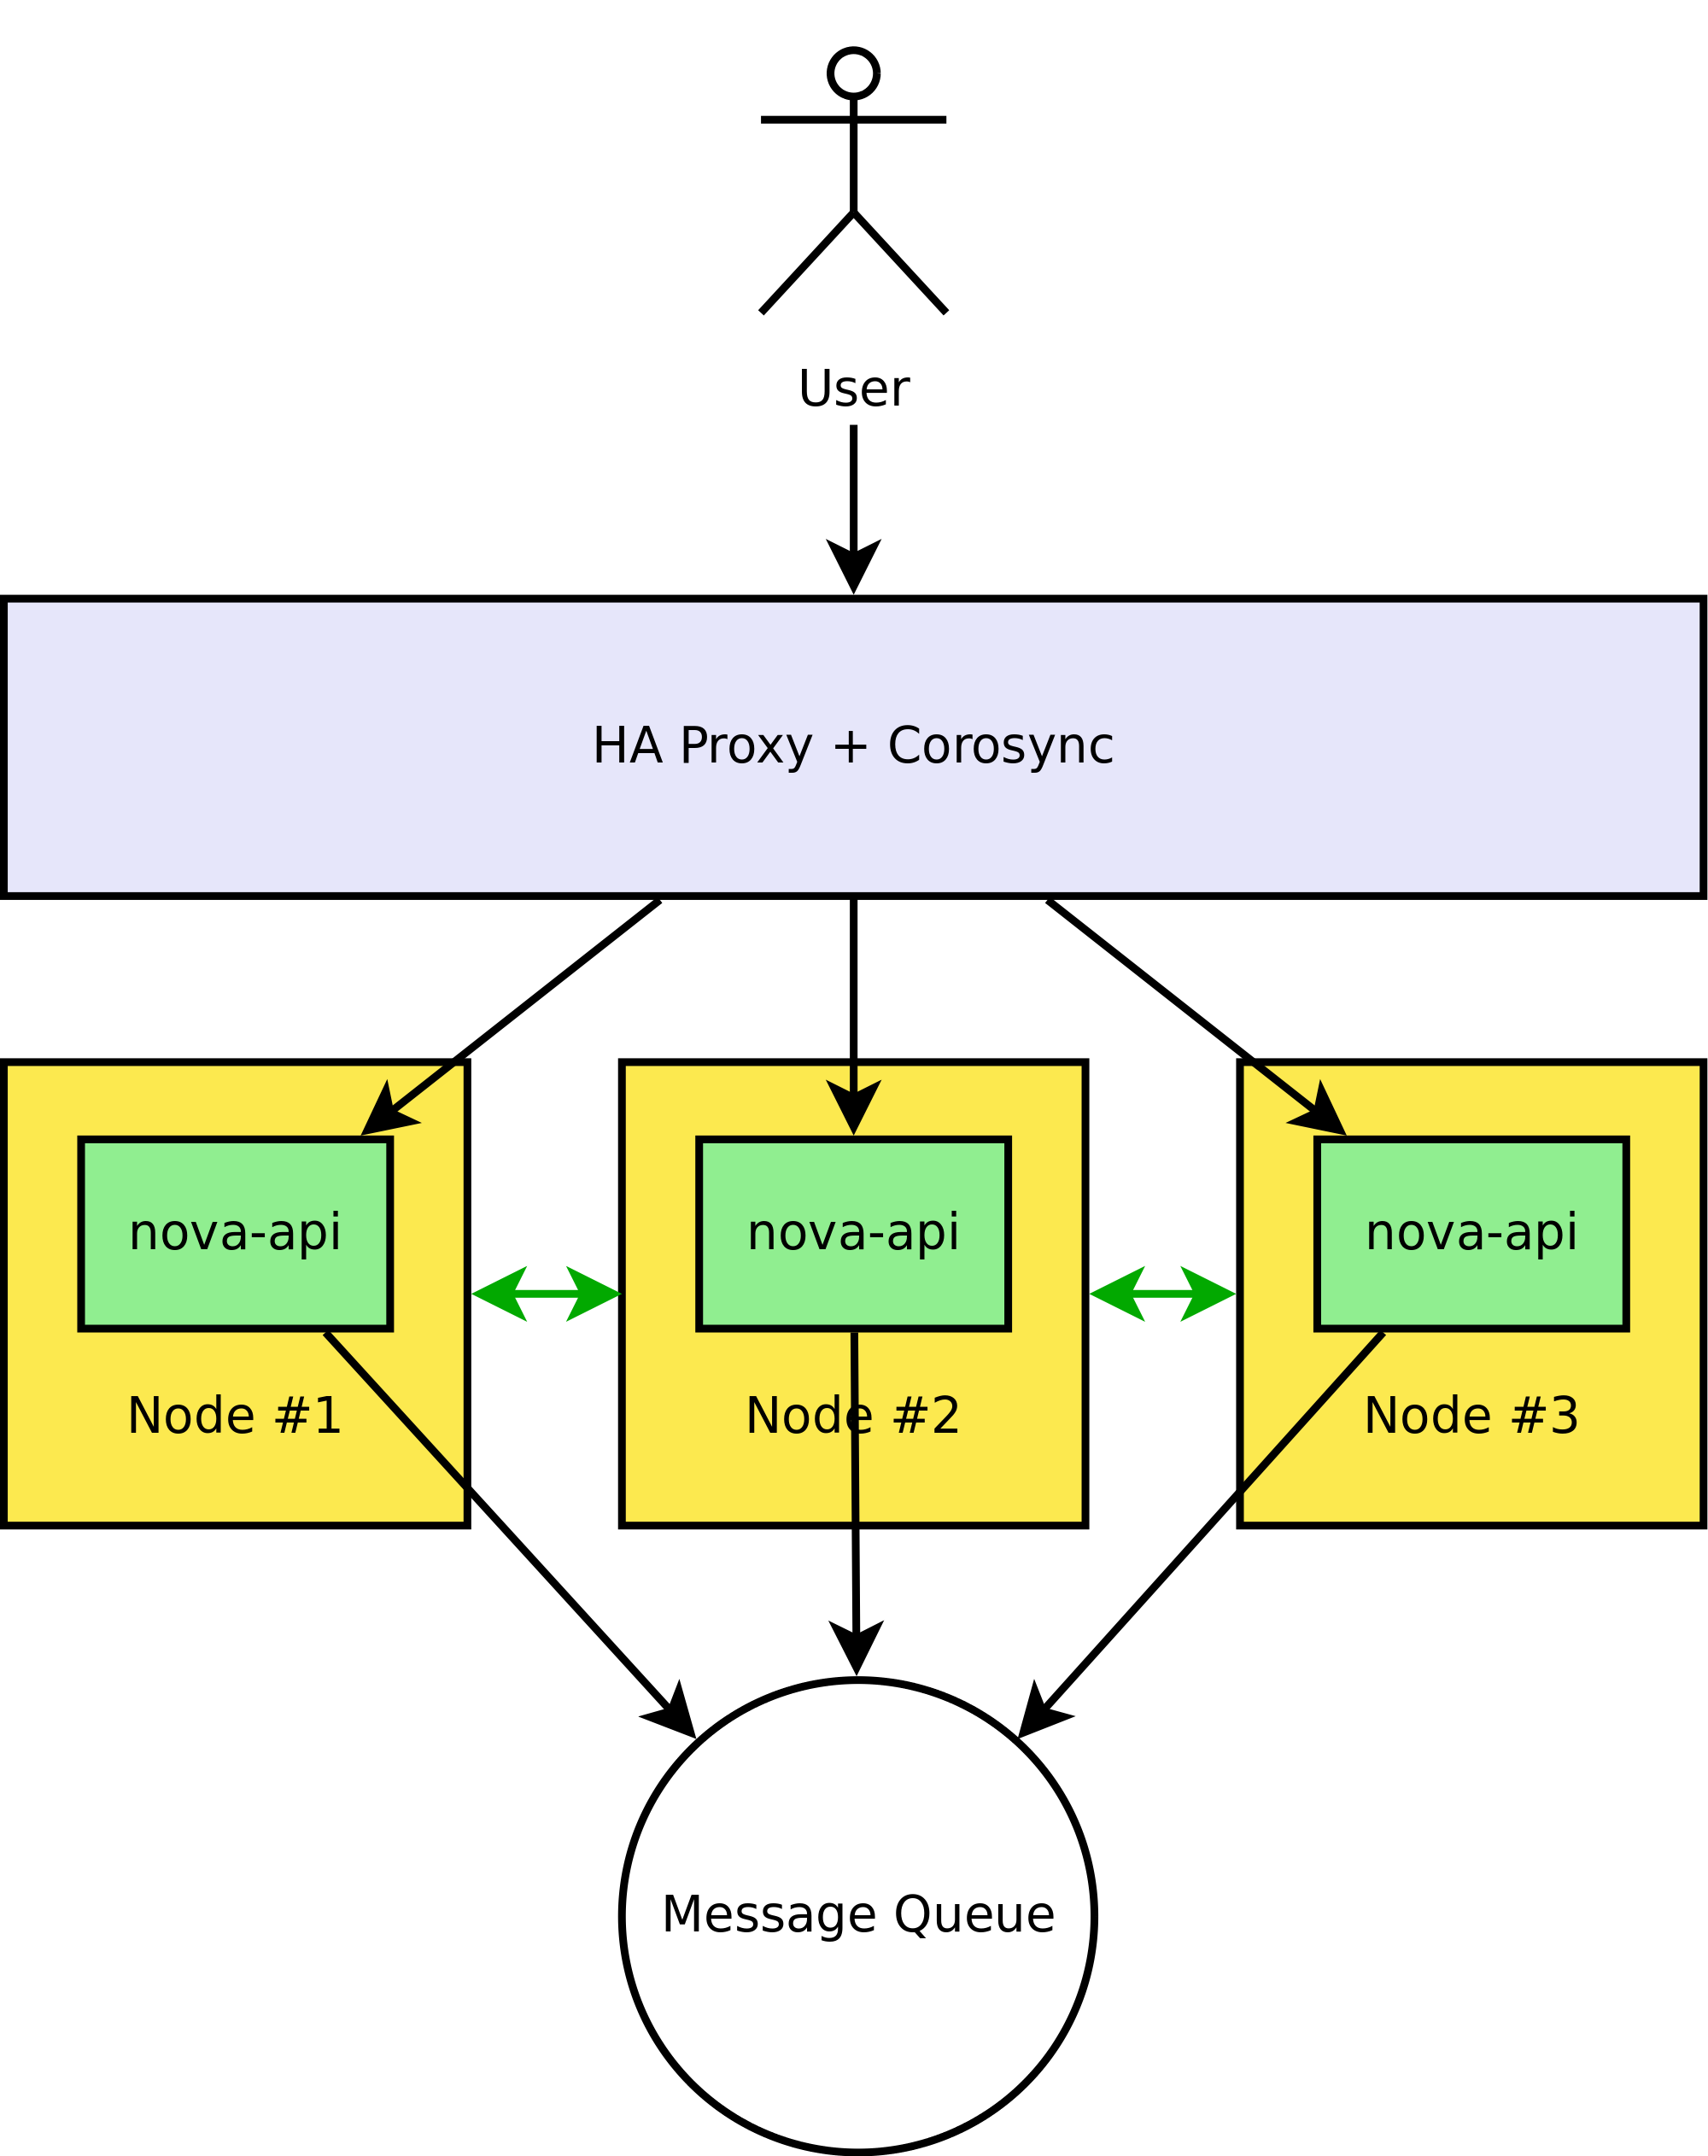
\includegraphics[height=7cm]{images/haproxy1.png}
    \end{center}
\end{frame}

\begin{frame}
    \frametitle{HAProxy + REST API}
    \begin{center}
        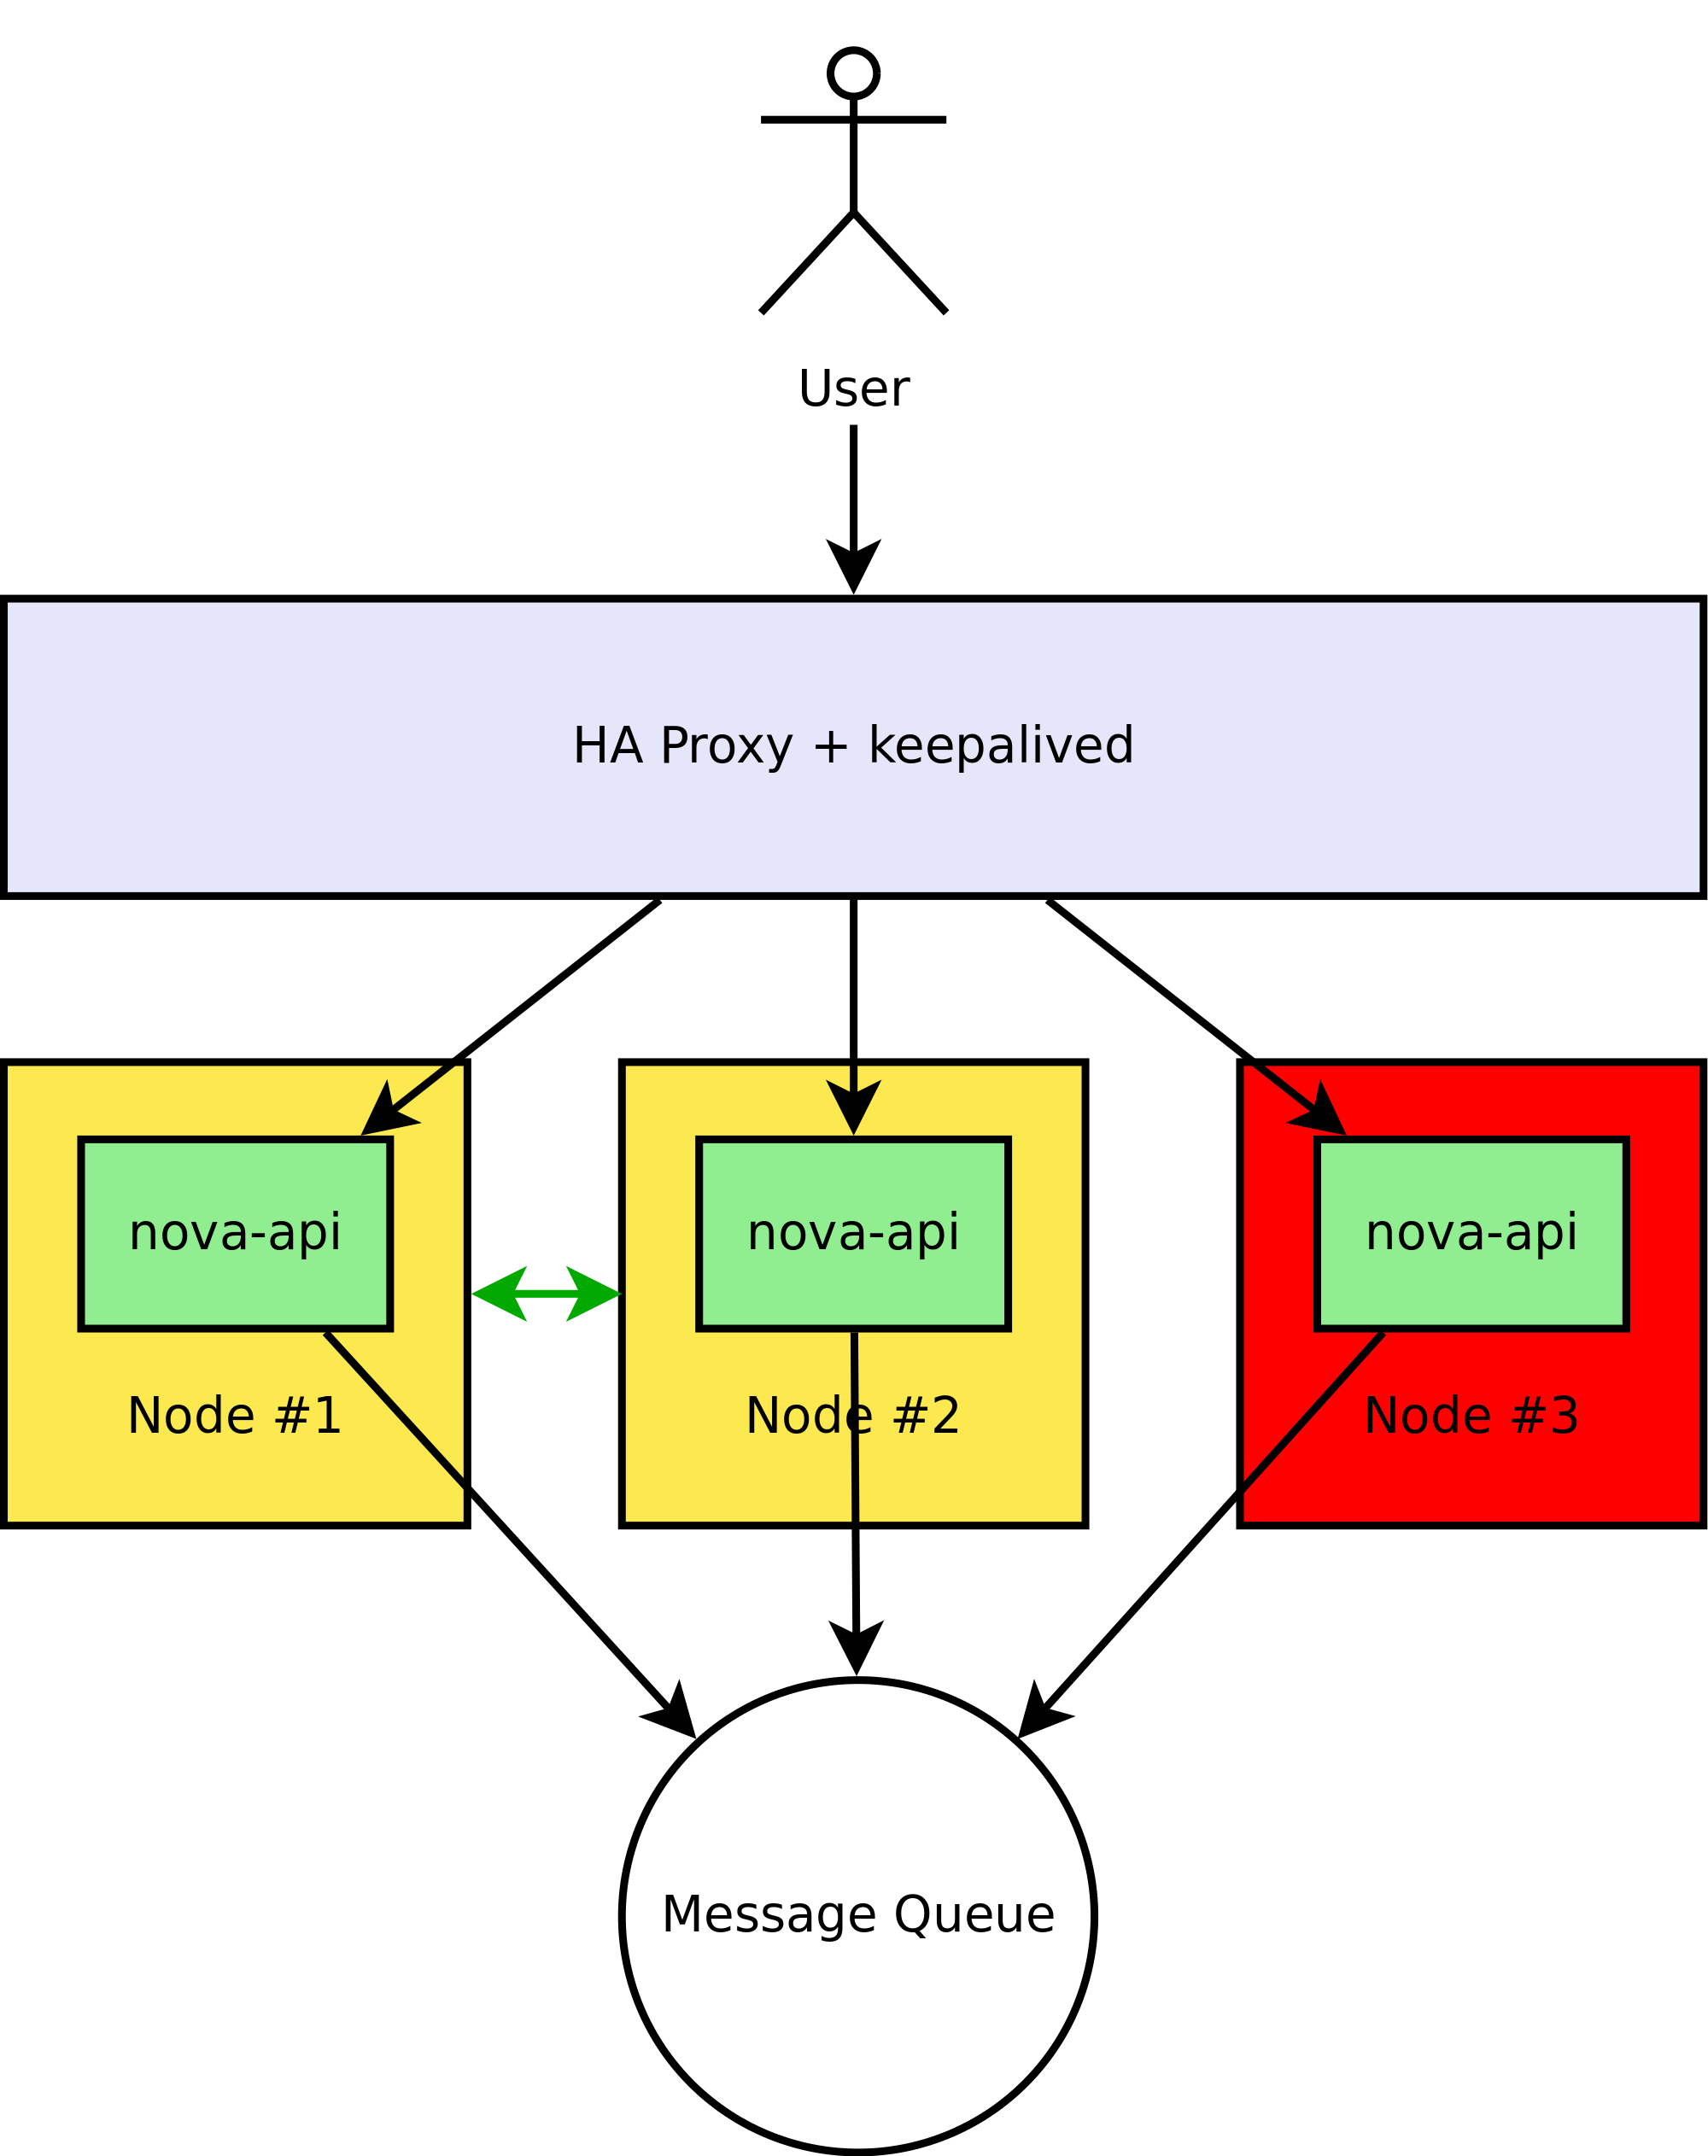
\includegraphics[height=7cm]{images/haproxy2.png}
    \end{center}
\end{frame}

\begin{frame}
    \frametitle{HAProxy + REST API}
    \begin{center}
        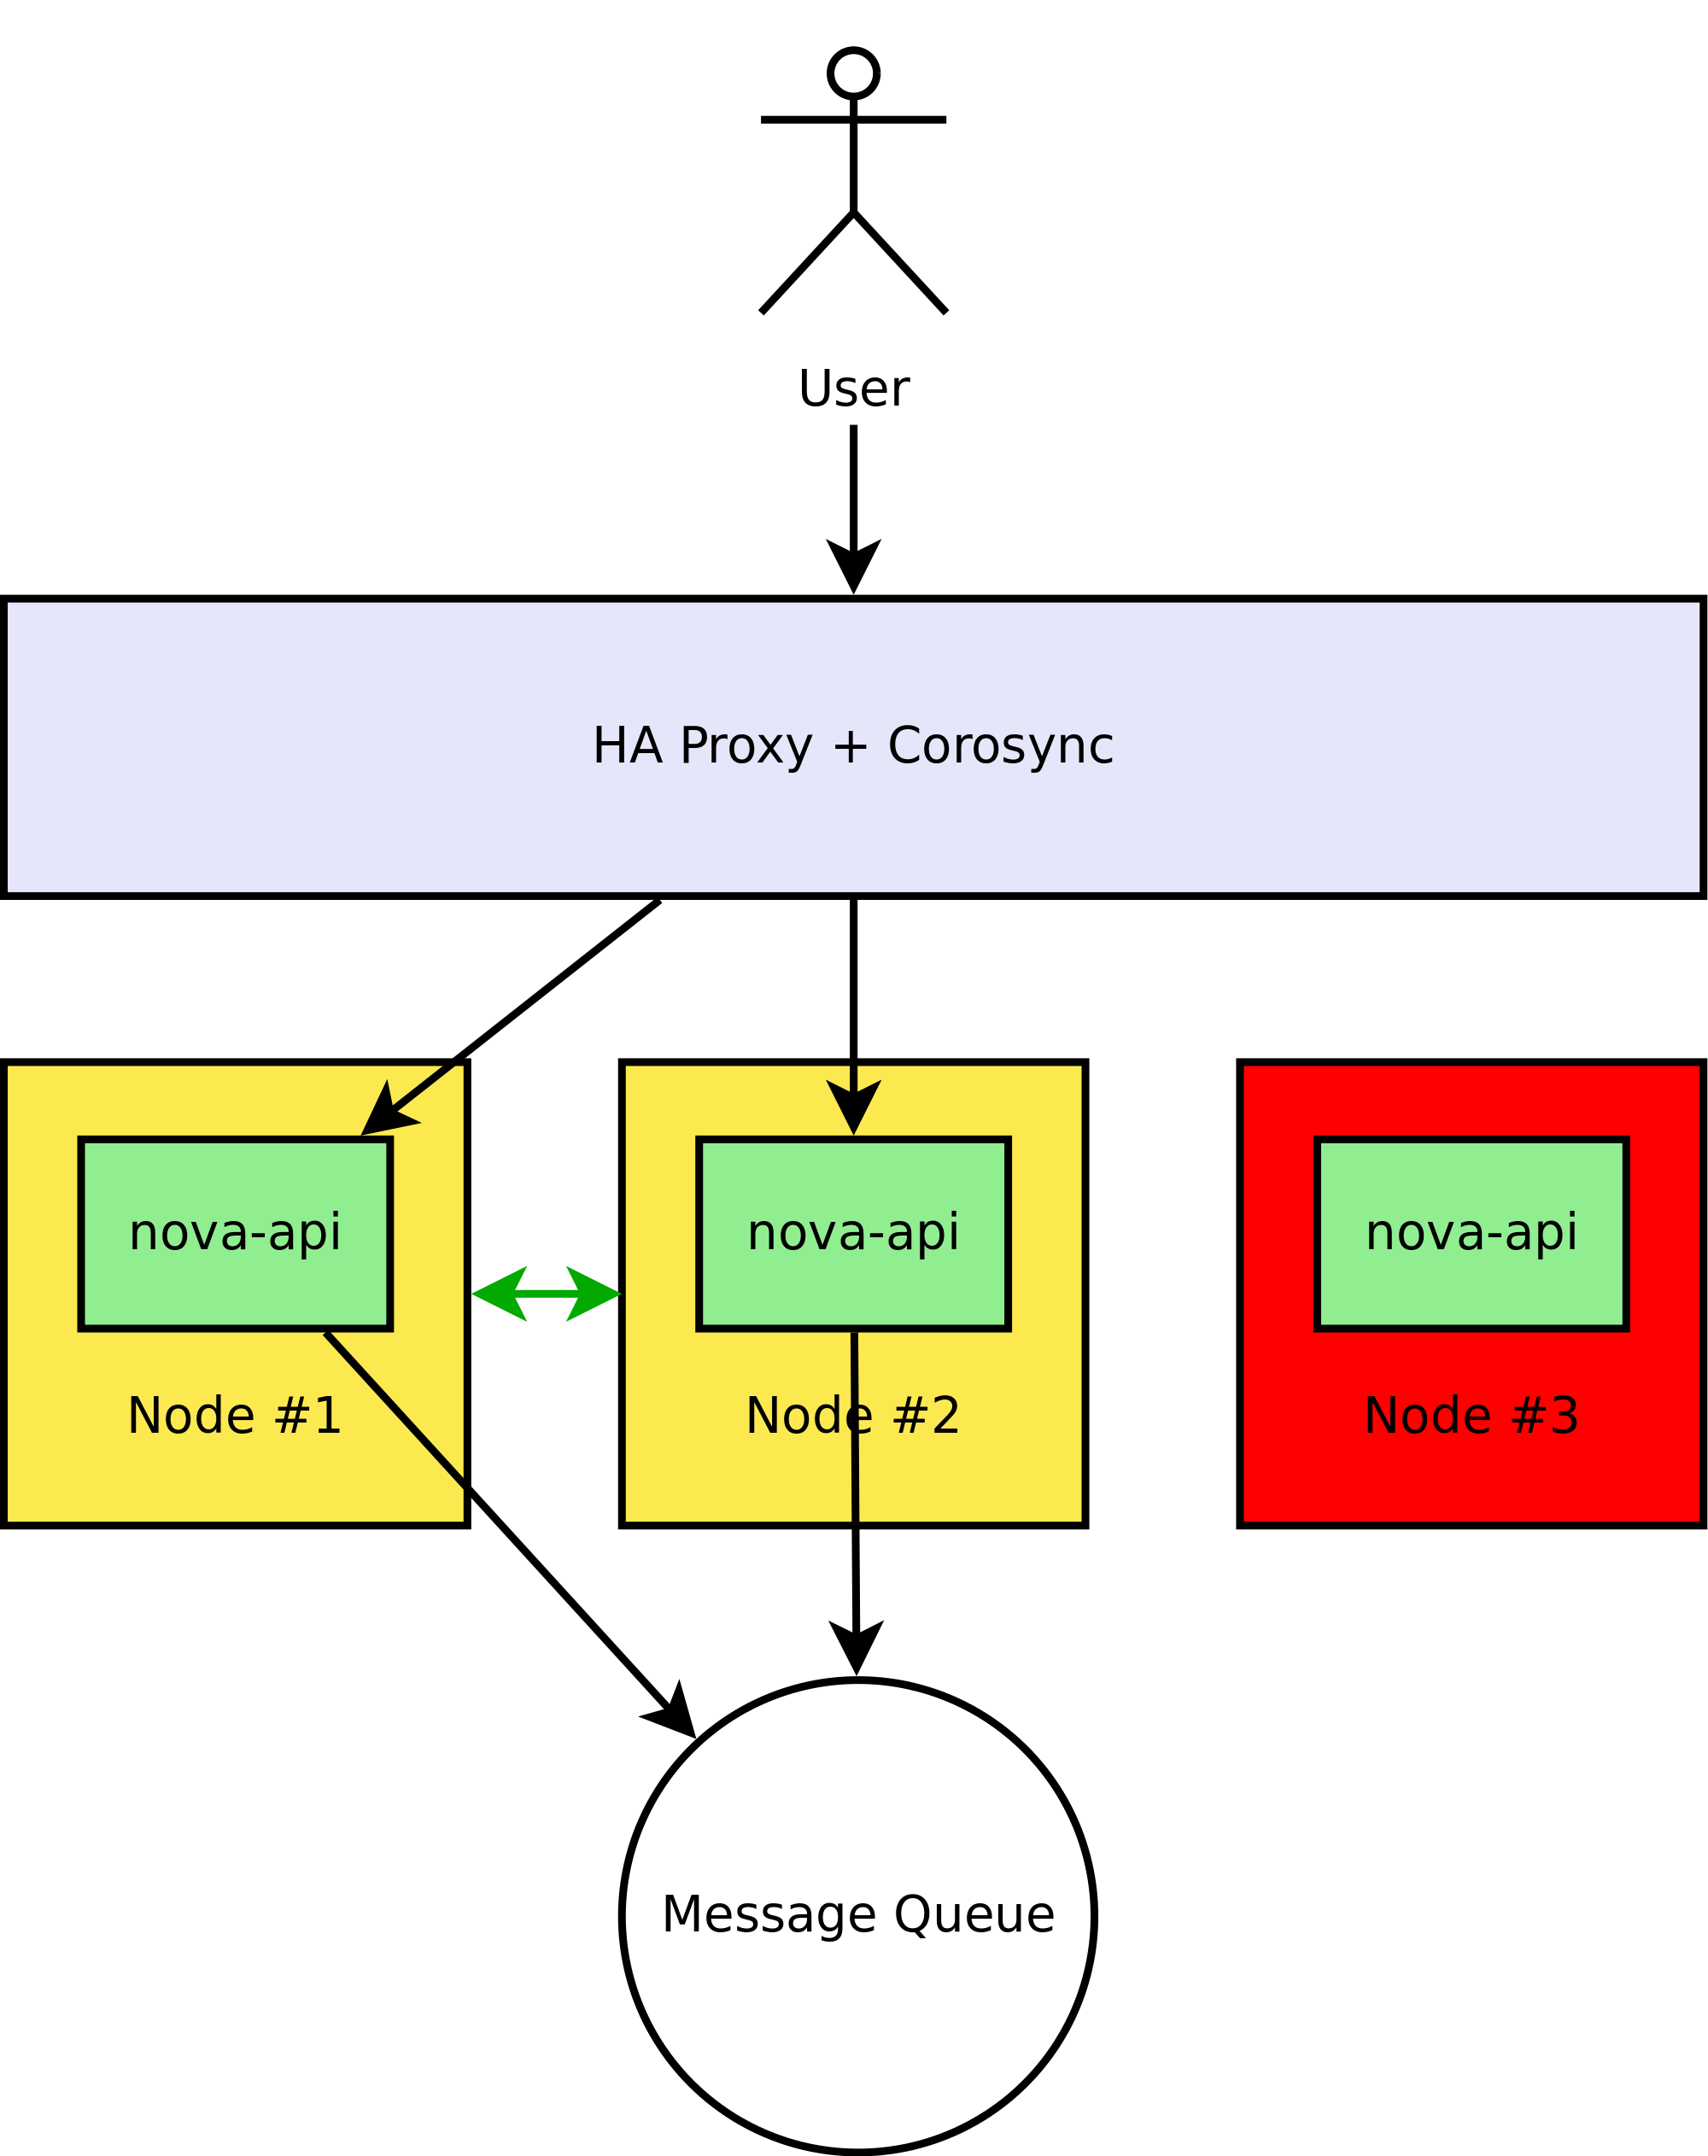
\includegraphics[height=7cm]{images/haproxy3.png}
    \end{center}
\end{frame}

\begin{frame}
    \frametitle{Message queue-bound services}
    \begin{itemize}
        \item If stateless - just run multiple of them on controller nodes in A/A mode.
        \pause
        \item If stateful - uh, oh…
        \pause
        \begin{itemize}
            \item You need to run it as A/P service…
            \pause
            \item …so you'll need some cluster management software like Pacemaker to monitor and keep it running…
            \pause
            \item …and some fencing software to protect from split-brains and zombie services.
        \end{itemize}
    \end{itemize}
\end{frame}

\begin{frame}
    \frametitle{Pacemaker 101}
    \begin{itemize}
        \item Distributed cluster management software
        \item Features include:
        \begin{itemize}
            \item awareness of other applications in the stack
            \item a shared quorum implementation and calculation
            \item data integrity through fencing
            \item automated recovery of instances to ensure capacity
        \end{itemize}
        \item Configurable and extendable through OCF (\emph{Open Cluster Framework}) agents/scripts.
        \item Pacemaker is rather heavy, so OpenStack projects are aiming to get as many services A/A capable.
    \end{itemize}
\end{frame}

\begin{frame}
    \frametitle{Fencing}
    \begin{itemize}
        \item In case of non-responding application we don't know if it's dead or a network partition occurred.
        \item To make sure that we won't have two A/P service instances running, we need to fence the node where dead service instance resides on.
        \pause
        \item Software solution: STONITH - \emph{Shoot The Other Node In The Head}.
        \begin{itemize}
            \item UPS (Uninterruptible Power Supply)
            \item PDU (Power Distribution Unit)
            \item Blade power control devices
            \item Lights-out devices
        \end{itemize}
        \item Be aware - this complicates the system even more!
    \end{itemize}
\end{frame}

\begin{frame}
    \frametitle{Neutron HA}
    \begin{itemize}
        \item Liberty
        \begin{itemize}
	        \item DVR - Distributed Virtual Router - east/west routing on compute node, floating IP resolved on compute node also. The SNAT (for fixed IP) is on centralized network node, only one network node can be available per installation
	        \item L3 HA - multiple network node in active/passive configuration (VRRP, keepalived) - this is single network node resolving east/west routing, floating and and SNAT on single node.
	        \item DHCP, metadata agents - A/A, multiple agents are working on each network node.
	    \end{itemize}
        \item Mitaka
        \begin{itemize}
            \item DVR-HA - Use DVR and multiple active/passive network nodes for SNAT.
        \end{itemize}
    \end{itemize}
\end{frame}

\begin{frame}
    \frametitle{Resources and further help}
    \begin{itemize}
        \item \href{http://docs.openstack.org/ha-guide/}{OpenStack High Availability Guide}
        \item \href{https://docs.mirantis.com/openstack/fuel/fuel-7.0/reference-architecture.html}{Mirantis OpenStack 7.0 Reference Architecture} (might be a little outdated)
        \item \href{http://clusterlabs.org/}{Pacemaker documentation}
        \item \href{http://docs.openstack.org/mitaka/networking-guide/scenario-dvr-ovs.html}{Neutron DVR Documentation}
        \item \href{http://docs.openstack.org/mitaka/networking-guide/scenario-l3ha-ovs.html}{Neutron L3 VRRP Documentation}
        \item \href{irc://chat.freenode.net/openstack-ha}{\#openstack-ha IRC channel (freenode)}
    \end{itemize}
\end{frame}

\begin{frame}
    \begin{center}
        \huge Thank you!

        \vfill

        \Large https://github.com/dulek/openstack-meetup-wroclaw-ha

        \vfill

        \small remind me to switch to next slide for Q\&A
    \end{center}
\end{frame}

\begin{frame}
    \frametitle{Legal Notices and Disclaimers}
    \begin{itemize}
\item Intel disclaims all express and implied warranties, including without
limitation, the implied warranties of merchantability, fitness for a particular
purpose, and non-infringement, as well as any warranty arising from course of
performance, course of dealing, or usage in trade.

\item Intel, the Intel logo and others are trademarks of Intel Corporation in the 
U.S. and/or other countries.

\item *Other names and brands may be claimed as the property of others.
    \end{itemize}
\end{frame}

\end{document}

